\section{Grappa} \label{sec:grappa}

\begin{figure}[t]
\begin{center}
  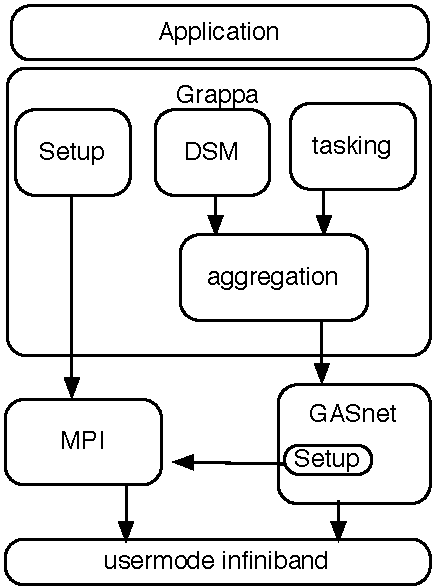
\includegraphics[width=0.5\columnwidth]{figs/grappa-crappy}
\begin{minipage}{0.95\columnwidth}
  \caption{\label{fig:grappa} Grappa runtime system \vspace{-4ex}}
\end{minipage}
\vspace{-3ex}
\end{center}
\end{figure}

In this section we describe the Grappa runtime system (Figure~\ref{fig:grappa}).  Grappa is a software runtime system that one adds to a commodity HPC cluster.  It provides the following software abstractions to applications: \textbf{memory}, a global distributed shared memory and \textbf{tasking}, co-operative multithreading with automatic load balancing.  Under the hood a third component, \textbf{communication}, a network packet scheduler/aggregator is key to achieving high performance, but largely invisible to applications.  We will now describe each of these components.

\subsection{Memory}

Applications written for Grappa utilize two forms of memory: local and global.

Local memory is exactly what its name implies.  Accesses occur through conventional pointers.  The compiler emits an access and the memory is manipulated directly.  Obviously, local pointers cannot access memory on other system nodes.  Applications use local accesses for a number of things in Grappa: the stack associated with a task, accesses to localized global memory in caches (see below), and accesses to debugging infrastructure that is local to each system node.

Global memory is a distributed block cyclic heap.  Applications allocate memory in this heap and a global pointer is returned.  Global pointers are utilized in one of two ways: (1) via a \emph{cache} or (2) via a \emph{delegate}.

\paragraph{Cache:} With a cache, applications can instruct Grappa to fetch a global pointer (of any length) and return a local pointer to a cached copy of the global memory.  Under the hood, Grappa performs the mechanics of gathering chunks of data from multiple system nodes and presenting a conventional appearing linear block of memory as a pointer into a cache.  Caches are either read-only or read-write and alternatively incoherent or coherent.  Read-only and and read-write caches are what their names imply.  Under the hood, the distinction between these two forms of caches lays in how they interact with the directories that maintain the coherence state for coherent access to the memory the global pointer points to.  For coherent caches, these directories maintain a simple coherence protocol that permits multiple outstanding read-only cached copies of data to exist, or alternatively, only a single outstanding read-write cached copy to exist.  Unlike hardware caches, these software caches require explicit release operations issued in software; i.e., applications must explicitly inform Grappa when the local pointer that points into a local cached copy of global memory is no longer needed.  Grappa then uses this release operation to interact with the directories that control the global memory in question.  For incoherent accesses, the directories are bypassed.  Applications acquire a local pointer to a cached copy of the global data and can expressly push the data from this local copy back to global memory in order to post any writes.  Obviously, applications should only use incoherent accesses when they can \emph{prove} accesses across multiple threads and system nodes are disjoint, or solely read-only, or (in rarer cases) maintaining a consistent view of memory is irrelevant to application correctness, or for debugging purposes.

\paragraph{Delegates:} Alternatively applications can dispatch computation to be performed on individual machine-word sized chunks of global memory to the memory system itself (e.g., \emph{fetch-and-add}).  Applications provide a pointer to a function and a global pointer to Grappa, which takes care to execute that function on the system node that actually stores the memory pointed to by the global pointer.  In such cases, localization of the pointer is more efficient.  Delegate operations are most often used for synchronization primitives, but really any computation is permissible.

\TODO{Check: Do delegate operations interact with the directories?  Are they coherent?}

Figure~\ref{fig:globalmemory} depicts the global memory architecture and access interface.

\subsection{Tasking}

Grappa provides its own task library to applications.  Applications begin execution with a single task, bound to an existing thread stack.  Tasks can spawn new tasks, and those new tasks are initially not bound to a thread stack, but instead are queued for future execution.

Grappa context switches between tasks non-preemptively.  Most calls into the Grappa library, however, do initiate a context switch, and tasks can explicitly yield control.  Grappa switches between tasks entirely within usermode, and in our experiments we have measured the context switch time to be only \checkme{40ns}.  This time is kept small because it is done entirely in usermode and only registers specified as caller saved by the compiler need be saved/restored.  Tasks become bound to a thread stack when no other task is runnable, or Grappa determines it is profitable to do so.  \TODO{How does Grappa determine this?}.

Tasks that are not bound to a stack are steelable by the work steeling system within Grappa.  This load balances work across the collection of nodes executing an application built on Grappa.  \TODO{Talk about the work steeling algorithm that we use}.

\subsection{Communication}

With Grappa, from the perspective of the application, all communication between tasks occurs through global shared memory.  These requests are ultimately translated into explicit inter system node communication requests that are dispatched to GASnet.  Under the hood there exists a key component within Grappa, the message aggregator, that makes fine-grained communication efficient on commodity Infiniband networks.  Infiniband achieves its peek bisection bandwidth \emph{only} when the packet sizes are relatively large (a kilobyte or more).  In our experience, graph algorithms request objects through the caching system (previously described) with a median object size of \checkme{16} bytes.  Our measurements, confirm manufactures published data~\cite{infinibandbandwidth}, that with this packet size the bisection bandwidth is only a small fraction, less than ~\checkme{5\%} of the peak bisection bandwidth.  The reason for this discrepancy is the combination of overheads associated with handling each packet (in terms of bytes that form the actual Infiniband packet, processing time at the card and processing on the CPU within the driver stack).

To work around this problem we perform packet aggregation.  Instead of dispatching a packet immediately to the Infiniband hardware, Grappa holds onto an individual communication request.  Pending requests that are to be sent to the same remote node are queued.  Once a sufficient number of them (in terms of bytes) or a timeout occurs, they are dispatched as a single packet to GASnet and onward to the Infiniband network.  In Section~\ref{sec:results} we explore the sensitivity of performance to these two key parameters, but the net result is that performance is maximized by aiming to aggregate for \checkme{1024} bytes and \checkme{1ms}.
